\chapter{Revisão Bibliográfica}
\label{ch:ch2}
Nesse capítulo são apresentadas as principais características das meta-heurísticas, com um foco maior no algoritmo escolhido para aplicação ao problema de DEP: os Algoritmos Genéticos. Além disso são discutidas também as características e dificuldades do gerenciamento de campos de petróleo, bem com uma revisão dos principais trabalhos que se propuseram a resolver o problema de DEP com o uso de meta-heurísticas.

\section{Meta-heurísticas}
\label{sec:section21}
Diariamente lidamos com uma série de problemas dos mais diversos tipos. Para \cite{Michalewicz2004}, um problema existe quando há uma diferença entre um estado atual e um estado no qual se deseja estar. Ainda segundo \cite{Michalewicz2004}, alocar recursos que estejam disponíveis para diminuir a diferença entre esses estados é o que chamamos de solução. É comum que exista mais de uma solução viável para a resolução de um problema, nesse caso, é sempre desejável que a solução ótima, ou a mais próxima disso, seja a escolhida para ser executada.

Nesse cenário, em que há diversas soluções candidatas para resolver um determinado problema, encontrar a solução ótima é um problema por si só. Esse problema em questão é conhecido como problema de otimização.  Tal otimização consiste em buscar pela solução ótima dentro de um conjunto de soluções (que formam o chamado espaço de busca), visando atender a algum critério. Geralmente tal critério é um determinado aspecto de interesse (objetivo) como lucro, desempenho, tempo ou distância, que deve ser maximizado ou minimizado. Na maioria das vezes é possível representar esse objetivo através de uma função matemática, conhecida como função objetivo e responsável por atribuir um número real a cada solução candidata do problema, indicando, dessa forma, o quão bem uma determinada solução resolve o problema.

São diversos os métodos que existem para resolver problemas de otimização. É possível partir para estratégias mais simples como a realização de uma busca por força bruta, enumerando e avaliando todas as soluções candidatas e escolhendo a melhor entre as opções, ou mesmo utilizar métodos mais clássicos como os baseados em gradiente. No entanto, a utilização de métodos como esses pode se mostrar ineficiente e até mesmo infactível, dependendo do problema que se deseja otimizar. \cite{Michalewicz2004} relatam algumas das características que tornam certos problemas de otimização difíceis de serem resolvidos:

\begin{itemize}
\item O problema possui uma quantidade grande de soluções candidatas;
\item O problema precisa ser simplificado para que se obtenha um conjunto de soluções candidatas. No entanto, as soluções geradas podem não ser boas o suficiente para solucionar o problema.
\item O problema possui restrições que exigem a realização de operações especiais para gerar soluções factíveis.
\end{itemize}

Problemas com essas características tornam inviável a avaliação de todas as soluções candidatas ou não permitem a definição de uma função objetivo que seja diferenciável, característica essencial para métodos baseados em gradiente, uma vez que esses métodos utilizam a derivada da função objetivo para direcionar a busca pela solução ótima. Para esse tipo de problema, é possível utilizar um grupo de métodos conhecidos por meta-heurísticas. 

Definir o que são meta-heurísticas não é uma tarefa simples. O termo foi vagamente introduzido por \cite{Glover1986} ao descrever a Busca Tabu como uma sobreposição de outra heurística. \cite{sorensen2013metaheuristics} propuseram uma definição mais concreta para o termo:


“Uma meta-heurística é uma estrutura algorítmica de alto nível e independente do problema que fornece um conjunto de orientações e estratégias para desenvolver algoritmos de otimização heurística. O termo também é utilizado para referir-se à implementação para um problema específico de tais algoritmos segundo as orientações destes” \cite{sorensen2013metaheuristics}.

De forma geral, é possível dizer que meta-heurísticas são metodologias de alto nível que podem ser usadas para desenvolver heurísticas a fim de resolver um problema específico de otimização \cite{Talbi2009}. Tais metodologias fazem parte de um campo maior de estudo conhecido por Otimização Estocástica \cite{Luke2013Metaheuristics}. A principal característica de algoritmos de otimização estocástica é o uso de técnicas que utilizam probabilidades para realizar operações durante o processo de busca por soluções ótimas. O uso de tal metodologia é comum em problemas de otimização para os quais nenhum outro método clássico pode ser aplicado com sucesso.

As meta-heurísticas tradicionalmente conseguem ser aplicadas a estes problemas por serem ferramentas de propósito geral que não exigem grandes adaptações, diferentemente de grande parte dos métodos clássicos de otimização. Ademais, as meta-heurísticas possuem estratégias que procuram escapar de soluções que representem ótimos locais do espaço de busca. Em contrapartida, principalmente pelo caráter estocástico destas metodologias, não há garantias de que a solução ótima, ou mesmo uma solução aceitável, será encontrada durante o processo de busca \cite{Talbi2009}. 

Apesar de não exigirem grandes adaptações, outros desafios surgem ao lidar com meta-heurísticas. Dentre eles, há a escolha de uma representação da solução candidata do problema, a definição da função objetivo a ser otimizada, as formas como as restrições do problema serão tratadas e a definição de parâmetros do algoritmo. Estes quatro pontos são detalhados a seguir.

\subsection{Representação da solução candidata}
\label{subsec:subc211}
A forma como uma solução candidata para o problema será representada computacionalmente ditará grande parte da estratégia de busca da meta-heurística, definindo diretamente o tamanho do espaço de busca que deve ser explorado e os operadores de busca que deverão ser utilizados. Uma solução candidata pode ser codificada de várias formas, sendo que grande parte dos problemas podem ter soluções representadas por codificações clássicas presentes na literatura, tais como cadeias binárias, vetores de valores discretos, vetores de valores reais ou permutações de valores inteiros. \cite{Talbi2009} sugere que uma representação da solução candidata deve possuir as seguintes características:

\begin{itemize}
\item \textbf{Plenitude:} relacionada à capacidade de a codificação representar toda as possíveis soluções para o problema.
\item \textbf{Conectividade:} diz respeito à vizinhança da solução. Deve existir um caminho entre duas soluções para que qualquer solução do espaço de busca possa ser obtida.
\item \textbf{Eficiência:} ditado pela facilidade de manipulação da solução pelos operadores de busca.
\end{itemize}

\subsection{Função Objetivo}
\label{subsec:subc212}
A função objetivo, ou função de avaliação, é o componente responsável por guiar o processo de busca de uma meta-heurística em direção à solução ótima do problema, visando atingir um objetivo determinado. Para cada solução candidata gerada durante o processo de busca, a função objetivo atribui um valor numérico indicativo da qualidade desta solução. Em alguns problemas, é comum que a própria formulação matemática do objetivo a ser atingido com a otimização do problema sirva como função objetivo, entretanto, existem casos nos quais não é possível definir uma formulação matemática explícita para o problema, como no problema de Definição de Estratégias de Produção (DEP) estudado neste trabalho. Para esses problemas é necessário recorrer a outras ferramentas para avaliação das soluções candidatas, como simuladores. Nesses casos, a função objetivo é uma função de caixa preta \cite{Talbi2009}. Em se tratando de meta-heurísticas, a definição de função objetivo geralmente é o único momento no qual se considera o conhecimento que se tem acerca do problema no processo de busca pela solução ótima.

\subsection{Definição de Parâmetros}
\label{subsec:subc213}
É comum a necessidade de definição de valores para uma série de parâmetros antes da aplicação de uma meta-heurística a um dado problema. Tais parâmetros controlam o funcionamento do algoritmo e têm grande influência no desempenho e na eficiência da busca pela solução ótima. Entretanto, a escolha dos valores ótimos destes parâmetros não é óbvia, além de tais valores não serem universais. A tarefa de ajustar os parâmetros depende bastante do problema ou, até mesmo, de uma instância do problema \cite{Talbi2009}.

Cada meta-heurística possui seu conjunto próprio de parâmetros a serem definidos, mas, de forma geral, tais parâmetros estão relacionados à quantidade de iterações do algoritmo e à probabilidade de um determinado operador ser executado. No caso de meta-heurísticas populacionais, ou seja, daquelas que trabalham simultaneamente com um conjunto de soluções candidatas, considera-se também importante a definição do número de soluções na população. Mais detalhes sobre os parâmetros utilizados para o algoritmo estudado serão dados no Capítulo 4.

\subsection{Tratamentos de Restrições}
\label{subsec:subc214}
É comum encontrar problemas em que nem todas as soluções candidatas podem ser implementadas com sucesso, por violarem uma ou mais restrições que, geralmente, são intrínsecas ao problema. Em um primeiro momento, considerar as restrições do problema no processo de busca pode ser vantajoso, uma vez que tais restrições limitam a quantidade de soluções possíveis, reduzindo o espaço de busca. No entanto, deve-se considerar que, ao reduzir o espaço de busca, pode-se dificultar o processo de geração de soluções que atendam às condições estabelecidas.

Sendo assim, cria-se a necessidade de que os operadores de busca sejam capazes de gerar soluções factíveis \cite{Michalewicz2004}, o que nem sempre é uma tarefa simples. Outra abordagem seria o uso de estratégias para lidar com soluções candidatas que violem uma ou mais restrições do problema, o que, segundo \cite{Talbi2009}, poderia ser feito da seguinte maneira:

\begin{itemize}
\item \textbf{Rejeição:} A forma mais simples de lidar com soluções infactíveis é rejeitá-las do processo de busca. Dessa forma, somente soluções factíveis são consideradas. Esta abordagem conservadora pode não ser eficiente quando o espaço de busca é limitado.
\item \textbf{Penalização:} Tais estratégias utilizam uma função de penalidade para atribuir uma penalização ao valor da função objetivo da solução infactível. O objetivo desta função é quantificar o quão infactível é a solução. Dessa forma, mesmo sendo infactível, as soluções não são descartadas de forma imediata do processo de busca.
\item \textbf{Reparação:} São estratégias que visam corrigir as soluções infactíveis, tornando-as factíveis. Geralmente estas estratégias utilizam heurísticas exaustivas para corrigir as soluções, sendo assim específicas para cada problema.
\item\textbf{Preservação de soluções factíveis:} Esta estratégia visa garantir que as soluções criadas sejam factíveis. Para tal, é necessário incorporar conhecimento específico do problema nos operadores de busca e na codificação da solução.

\end{itemize}

\subsection{Classificação das Meta-Heurísticas}
\label{subsec:subc215}
A quantidade de meta-heurísticas disponíveis na literatura é vasta, o que levou à utilização de vários critérios para a classificação destes algoritmos. Tais critérios podem ser vistos em \cite{Blum2003}, \cite{Talbi2009} e \cite{Boussaid2013}. De forma geral, as meta-heurísticas podem ser classificadas levando-se em consideração algumas de suas características, tais como a inspiração para a criação do algoritmo (inspirados ou não por eventos naturais), a forma com que elas lidam com as informações extraídas durante o processo de busca (com memória ou sem memória) ou a maneira como exploram o espaço de busca.

Esta última característica é um grande dilema ao projetar uma meta-heurística. Se por um lado, deseja-se diversidade nas soluções ao percorrer o espaço de busca (para que se tenha uma maior exploração do espaço), por outro deseja-se também uma boa capacidade de refinamento de soluções promissoras (explotação). Tal dilema é traduzido na forma como as meta-heurísticas gerenciam as soluções candidatas, sendo possível percorrer o espaço de busca com uma única solução (meta-heurísticas baseadas em solução única) ou com um conjunto de soluções (meta-heurísticas populacionais).

\subsubsection{Meta-heurísticas baseadas em solução única}
\label{subsec:subc2151}
As meta-heurísticas de solução única trabalham fortemente com o conceito de vizinhança. Ao menos para problemas de otimização combinatória, a vizinhança de uma solução s pode ser definida como o conjunto de soluções s', sendo que a distância entre s e s' deve ser menor ou igual a um limite de distância $\epsilon$ \cite{Talbi2009}. A forma como obtém-se a distância entre duas soluções e qual o valor ideal de $\epsilon$, no entanto, depende da representação da solução candidata e do problema em questão.

Sendo assim, o processo de busca por uma solução ótima das meta-heurísticas de solução única consiste, primariamente, em refinar uma solução inicial buscando melhorias através da vizinhança desta solução, priorizando desta forma a explotação do espaço de busca. Ainda assim, algumas meta-heurísticas possuem mecanismos para evitar que suas soluções fiquem presas em soluções de mínimo local. Conforme visto em \citeonline{Blum2003}, \citeonline{Talbi2009} e \citeonline{Boussaid2013} temos como exemplo de algoritmos deste grupo o Simulated Annealing (SA), Busca Tabu, Greedy Randomized Adaptive Search Procedure (GRASP), Variable Neighborhood Search, Busca Local Guiada e Busca Local Iterada.

\subsubsection{Meta-heurísticas populacionais}
\label{subsec:subc2152}
Ao contrário das meta-heurísticas baseadas em solução única, as meta-heurísticas populacionais lidam com um conjunto soluções candidatas (ou população). Existem duas abordagens para lidar com uma população de soluções \cite{Freitas2003,Ishibuchi1997}: a abordagem Pittsburgh, na qual cada elemento (indivíduo) do conjunto representa uma solução candidata ao problema; e a abordagem Michigan, onde a população como um todo representa a solução. Na abordagem Michigan é necessário, no entanto, que o problema possa ser decomposto em partes menores e que seja possível a avaliação destas partes.

Independentemente da abordagem utilizada, as meta-heurísticas populacionais buscam melhorar os indivíduos da população realizando interações entre esses indivíduos, seja através de combinações entre eles, aplicando mutações ou realizando buscas locais, utilizando membros como ponto de referência para os demais indivíduos ou, ainda, combinando esforços entre os indivíduos para atingir o objetivo desejado. Meta-heurísticas populacionais procuram manter diversidade entre as soluções, com o objetivo de explorar melhor o espaço de busca. Como exemplos de meta-heurísticas populacionais temos a Programação Evolutiva (PE), Algoritmos Genéticos (AG), Estratégias Evolutivas (EE) e Otimização por Colônia de Formigas (ACO, do inglês Ant Colony Optimization), apresentados por \citeonline{Blum2003}, \citeonline{Talbi2009} e \citeonline{Boussaid2013}.\citeonline{Boussaid2013} dividem as meta-heurísticas populacionais em dois grupos, (i) inspirados em computação evolutiva e (ii) inspirados em inteligência de enxame. 

\textbf{Computação Evolutiva}

Os algoritmos inspirados em computação evolutiva, de forma geral, trabalham com a ideia de evoluir a estrutura da solução através de operadores de seleção, recombinação e mutação que são aplicados aos indivíduos da população. O operador de seleção é um dos principais componentes dos algoritmos evolutivos, sendo responsável por levar a busca a soluções melhores (Talbi, 2009). Isto acontece pelo fato de tal operador ser encarregado de selecionar as soluções de melhor qualidade para permanecer na população ou para gerar novos indivíduos através do operador de recombinação e/ou mutação. 

Os algoritmos de computação evolutiva são inspirados em teorias evolutivas \cite{Talbi2009} como a teoria proposta por Darwin \cite{Darwin1859}, no qual os individuais mais bem adaptados ao ambiente tendem a sobreviver. Aqui o ambiente é o problema que se deseja resolver e o indivíduo melhor adaptado a este ambiente é a solução candidata que melhor resolve o problema. A função objetivo também é comumente conhecida por função de fitness e a qualidade de uma solução candidata também é denominada fitness desta solução.

Os algoritmos AG, EE e PE, apresentados em \citeonline{Blum2003} e também vistos em \citeonline{Talbi2009} e \citeonline{Boussaid2013}, fazem parte deste grupo. Além destes, \citeonline{Boussaid2013} apresentam como parte deste grupo: Programação Genética, Algoritmos de Estimação de Distribuição, Evolução Diferencial, Algoritmos Co-evolutivos e Algoritmos Culturais. Estes algoritmos também podem ser vistos em \citeonline{Talbi2009}. 

\textbf{Inteligência de Enxame}

Os algoritmos inspirados por inteligência de enxame buscam simular o comportamento social de um grupo de indivíduos. A principal característica dessa abordagem é o fato que de cada indivíduo é um agente simples, pouco sofisticado, que coopera com os demais indivíduos para que se movimentem no espaço de busca \cite{Talbi2009}. Os principais algoritmos deste grupo, apresentados por \citeonline{Talbi2009} e \citeonline{Boussaid2013}, são o ACO e Otimização por Enxame de Partículas (PSO, do inglês Particle Swarm Optimization). \citeonline{Boussaid2013} inclui ainda Bacterial Foraging Optimization Algorithm e Colônia de Abelhas Artificiais (ABC, do inglês Artificial Bee Colony) como parte deste grupo.

\subsection{Algoritmos Genéticos}

Dentre as meta-heurísticas apresentadas anteriormente, os Algoritmos Genéticos foram os escolhidos para a resolução do problema de DEP. AGs são algoritmos de busca inspirados pelos mecanismos da seleção natural e princípios de genética \cite{Goldberg1989}. Ainda segundo \citeonline{Goldberg1989}, a combinação entre a sobrevivência do indivíduo mais apto e a troca estruturada, e aleatória, de características entre os indivíduos tornam o AG um algoritmo robusto de busca. Ademais, a simplicidade do processo e sua eficiência são duas das principais características que tornam algoritmos genéticos tão atrativos e permitem usá-los para resolver os mais diversos tipos de problemas, que vão desde problemas mais clássicos, como o problema do caixeiro viajante \cite{Grefenstette1985}, até problemas mais sofisticados como o controle de tráfego aéreo \cite{Sergeeva2017}. 

A terminologia utilizada nesses algoritmos também é fortemente inspirada na biologia. Por exemplo, a estrutura do indivíduo (a solução candidata) aqui é chamada de cromossomo, o valor de cada variável que compõe o cromossomo é denominado alelo e cada variável pode ser chamada de lócus ou mesmo gene \cite{Back1997}.

Proposto por \citeonline{Holland1992}, na Universidade de Michigan, com o objetivo de abstrair e explicar o processo adaptativo da seleção natural e, também, de desenvolver sistemas artificiais que possuam características importantes da seleção natural, os algoritmos genéticos consistem em, a cada iteração (ou geração), produzir uma nova população de indivíduos através do uso de três operadores: seleção, recombinação (ou crossover) e mutação. Mais detalhes sobres os três operadores são dados nos tópicos a seguir. A Figura \ref{fig:fig2-1} apresenta um fluxograma da estrutura geral de um algoritmo genético. 

\begin{figure}[htb]
\centering
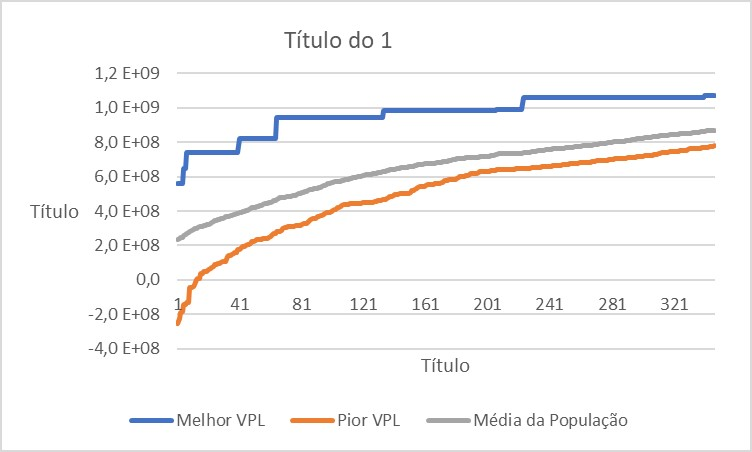
\includegraphics[scale=0.25]{1}
\caption{Fluxograma apresentando a estrutura geral de um algoritmo genético.}
\label{fig:fig2-1}
\end{figure}

\subsubsection{Operador de seleção}
O operador de seleção possui um papel importante no desempenho do algoritmo genético, uma vez que esse é o operador responsável por selecionar os indivíduos que farão parte do processo de recombinação.  Aqui é utilizada a analogia da seleção natural (Goldberg, 1985), em que indivíduos com fitness melhores têm mais chances de serem selecionados. Um exemplo de operador clássico que utiliza dessa lógica é a Seleção por Roleta \cite{Talbi2009, Kacprzyk2015, Luke2013Metaheuristics}.

No entanto, apesar de ser desejável que soluções melhores sejam selecionadas para que possam gerar soluções ainda mais promissoras, pode acontecer de tal pressão seletiva levar a uma população com pouca, ou nenhuma, diversidade. Dessa forma o algoritmo pode convergir para um ponto do espaço de busca de forma prematura. Sendo assim, alguns operadores de seleção utilizam estratégias diferentes para lidar com a tarefa de selecionar um indivíduo da população, seja manipulando o fitness para uma distribuição de probabilidades mais equilibrada, como a Seleção por Ranqueamento \cite{Talbi2009, Kacprzyk2015}, ou realizando competições entre os indivíduos e selecionando aquele com melhor desempenho como a Seleção por Torneios \cite{Talbi2009, Kacprzyk2015}. 

\subsubsection{Operador de recombinação}
A recombinação é um dos recursos que mais distingue algoritmos genéticos das outras meta-heurísticas \cite{Luke2013Metaheuristics}. Esse é o operador responsável por gerar novos indivíduos que possivelmente farão parte da população do algoritmo. O operador realiza a combinação de dois ou mais indivíduos para a criação de pelo menos um novo indivíduo. Espera-se que a combinação de partes dos indivíduos pais acabe por gerar descendentes que sejam melhores que os indivíduos originais \cite{Kacprzyk2015} e que mantenham parte das características de cada pai.

A forma como as combinações entre os indivíduos selecionados é realizada varia conforme a codificação escolhida. Para codificações baseadas em vetor, como a cadeia binária, é comum o uso de um dos de três operadores clássicos para essa tarefa: o Crossover de Um Ponto, de 2-Pontos e o Crossover Uniforme \cite{Talbi2009}. O operador de 1-Ponto seleciona aleatoriamente uma posição da cadeia e troca todos os valores do cromossomo entre indivíduos que estiverem abaixo dessa posição.  A mesma lógica é utilizada pelo operador de 2-Pontos, a diferença aqui é que duas posições são escolhidas e os valores entre as posições são trocados entre os indivíduos. Por fim, o operador de Recombinação Uniforme escolhe aleatoriamente, para cada um dos valores do cromossomo, o valor de um dos indivíduos selecionados para a recombinação. A Figura \ref{fig:fig2_2} ilustra o funcionamento desses três operadores.

\begin{figure}[htb]
\centering
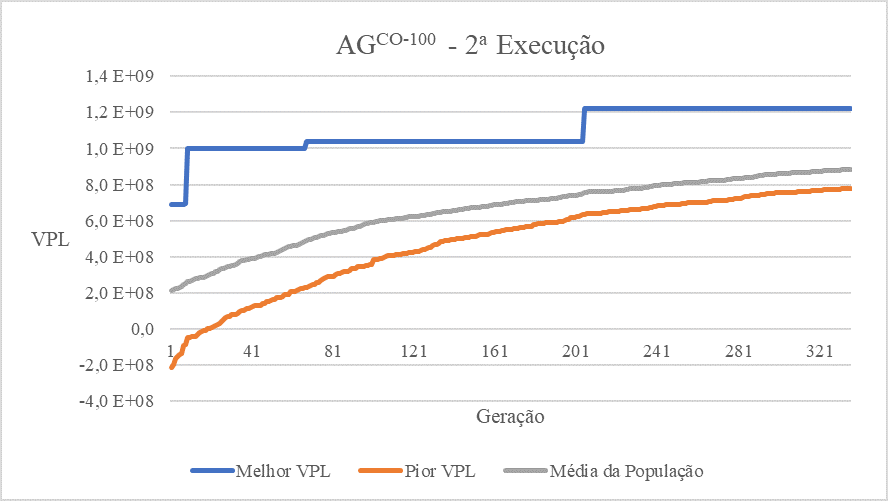
\includegraphics[scale=1]{2}
\caption{Exemplo ilustrando o funcionamento dos operadores de Crossover de 1-Ponto, Crossover de 2-Pontos e Crossover Uniforme.}
\label{fig:fig2_2}
\end{figure}

Já para soluções representadas através de codificações de valores reais, os operadores são divididos em dois grupos: (i) recombinação centrada na média e (ii) recombinação centrada nos pais \cite{Talbi2009}. No primeiro grupo os indivíduos são gerados com base no centroide dos pais, sendo o Crossover Simplex \cite{Tsutsui1999} e o Crossover Geométrico \cite{Michalewicz1996} são exemplos de operadores que utilizam essa estratégia. Já o segundo grupo procura gerar indivíduos que façam parte da vizinhança dos pais, dessa forma os novos indivíduos serão semelhantes aos pais que os geraram: o Crossover Binário Simulado \cite{Deb1994} é um exemplo de operador desse grupo.   

Independentemente da codificação escolhida, dois pontos devem ser levados em consideração ao se definir, ou mesmo desenvolver, um operador de recombinação: (i) hereditariedade e (ii) validade \cite{Talbi2009}. O primeiro diz respeito à capacidade do operador de preservar as características dos indivíduos “pais” ao gerar um indivíduo descendente. Já a validade é a capacidade do operador de gerar um indivíduo válido, ou seja, uma solução factível para o problema. Essa característica pode tornar-se difícil de atingir em problemas onde diversas restrições devem ser consideradas durante o processo de otimização.

\subsubsection{Operador de mutação}

Apesar dos operadores de seleção e recombinação terem um papel primário no processo de busca dos algoritmos genéticos, esses operadores, ocasionalmente, podem acabar levando à perda de características importantes dos indivíduos \cite{Goldberg1989}. Sendo assim, o operador de mutação permite contornar essas perdas realizando pequenas variações no cromossomo de um determinado indivíduo. Tal operação ainda permite explorar pontos do espaço de busca que, sozinho, o operador de recombinação pode não ser capaz de atingir.

Assim como o operador de recombinação, o operador de mutação também deve se preocupar em gerar indivíduos válidos. \cite{Talbi2009} ainda afirma que tal operador deve ser capaz alcançar qualquer ponto do espaço de busca e as alterações realizadas devem ser controladas. A forma mais comum de se controlar tal operação é atribuir uma probabilidade consideravelmente baixa para que o operador seja executado.

A mutação de um indivíduo também varia conforme a codificação escolhida para seu cromossomo. No entanto, a ideia geral do operador de mutação é variar de forma aleatória os valores do cromossomo de um indivíduo. 

\subsubsection{Manutenção da População}

Como já foi abordado anteriormente, algoritmos genéticos lidam com uma população de soluções. Sendo assim, a estratégia utilizada por tais algoritmos para a manutenção dessa população é um tópico que merece atenção. Há duas estratégias bastante difundidas na literatura para tal manutenção, tais estratégias recebem os nomes de Geracional e Regime Permanente \cite{Kacprzyk2015}.

Na estratégia Geracional, uma nova população é criada a cada geração. Isso é feito selecionando-se um par de soluções e gerando novos indivíduos até que a nova população esteja completa. Tal estratégia pode levar a uma perda prematura dos melhores indivíduos, já que existe a possibilidade desses indivíduos não serem selecionados para o processo de recombinação e passarem suas características a próxima geração. Uma forma de contornar esse problema é garantir que os k melhores indivíduos de uma população de tamanho n estejam na nova população, sendo assim serão gerados somente n-k novos indivíduos para a próxima geração. Essa abordagem é conhecida como Elitismo \cite{Talbi2009}, sendo os k elementos denominados Elite.

A estratégia de Regime Permanente apresenta uma abordagem mais conservadora de manutenção da população. Enquanto a estratégia Geracional atualiza toda a população a cada geração, aqui uma quantidade restrita de indivíduos é criada a cada geração (geralmente um ou dois, dependendo do operador de recombinação escolhido) e são inseridos na população substituindo algum indivíduo. É comum que os novos indivíduos substituam os piores indivíduos da população, caso sejam melhores que esses. No entanto, outas regras podem ser utilizadas para esse processo, como a substituição de um dos indivíduos que participaram da recombinação ou, ainda, a escolha aleatória de um elemento da população para ser substituído.

Nesse trabalho os AGs, tanto em versão geracional quanto de regime permanente, foram utilizados para a resolução do problema de DEP.  Em um primeiro momento foram utilizadas as versões clássicas dessas duas variações do AG e dos operadores de seleção, recombinação e mutação. Em um seguida os AGs aqui estudados foram utilizados como base para o desenvolvimento de uma versão modificada que apesente um melhor desempenho para a resolução do problema. O mesmo foi feito com os operadores de recombinação e mutação, além da inclusão de um operador de busca local. Mais detalhes são apresentados no Capítulo 3.

\section{Gerenciamento de campos de petróleo}
\label{sec:section22}
Desenvolver e gerenciar campos de petróleo é uma tarefa que traz uma série de desafios, associados, dentre outros, à aquisição de dados sísmicos — visando o mapeamento inicial da região de um campo em potencial —, à modelagem geológica, à definição da estratégia de produção a ser adotada pela empresa exploradora do campo e à adequação dos processos adotados para o atendimento das regulamentações ambientais \cite{Morais2013}. Ainda, são altos os investimentos necessários para tal atividade e a tomada de decisão durante esse processo torna-se de alto risco devido ao elevado grau de incertezas envolvidas.

Dentre as incertezas relacionadas ao problema podemos citar: (i) as incertezas geológicas, relacionadas às propriedades físicas do reservatório de petróleo, como porosidade e permeabilidade; (ii) as econômicas, que dizem respeito à dinâmica do mercado e são associadas às flutuações no preço futuro do petróleo, nas taxas de juros e nos valores de câmbio; e (iii) as operacionais, tais como eventuais quebras de equipamentos. Tais incertezas têm um impacto direto na tomada de decisão e, por conta dos altos investimentos envolvidos nessa atividade, são diversos os trabalhos que se focam em encontrar métodos para reduzir tais incertezas \cite{Oliveira2017,Maschio2010, Silva2012}.

A fim reduzir a complexidade durante o desenvolvimento e gerenciamento de campos de petróleo, \citeonline{Schiozer2015} propuseram uma metodologia composta de doze etapas, integrando análise de risco, ajuste de histórico, técnicas para redução de incerteza e seleção de estratégia de produção. A seguir um resumo das doze etapas estabelecidas.

\begin{enumerate}
\item Caracterização do reservatório sob incerteza;
\item Construção e calibração do modelo de simulação;
\item Verificação de inconsistências no caso base;
\item Construção de cenários considerando todos os cenários possíveis;
\item Redução do número de cenários através de dados dinâmicos;
\item Seleção de uma estratégia de produção para o caso base;
\item Geração da primeira estimativa da curva de risco;
\item Seleção de modelos representativos;
\item Seleção de uma estratégia de produção para cada modelo representativo;
\item Seleção de estratégia de produção considerando incertezas;
\item Identificação de potenciais mudanças na estratégia de produção que possam gerar mais chances de sucesso;
\item Definição da curva de risco final e tomada de decisão a respeito do campo. 

\end{enumerate}

Dentre as etapas listadas, o planejamento da estratégia para extração de petróleo (ou estratégia de produção), referente às etapas 6, 9 e 10, é particularmente relevante, uma vez que tal estratégia deverá ser adotada, pelo menos em sua essência, durante todo o período em que o campo será explorado. \citeonline{Barreto2014} ainda ressalta que esta etapa de planejamento é o momento que necessita de maior esforço, isso porque os problemas de engenharia são de maior escala e envolvem mais riscos e recursos financeiros.

\subsection{Estratégia de produção }

Em Engenharia de Reservatórios, estratégia de produção é o termo utilizado para referir-se às características operacionais e de infraestrutura do sistema de produção que será utilizado para a exploração do campo de petróleo. Tal sistema é composto por uma série de processos e equipamentos. 

Dentre todos os processos que o sistema de produção envolve, \citeonline{Figueira2014} cita como sendo os principais: o processo de recuperação, que consiste na metodologia para extração dos fluidos das rochas do reservatório; o sistema de elevação e escoamento, pelo qual o fluido é transportado dos poços até a superfície; e o processamento primário de produção, que corresponde a uma série de processos que visam separar os diferentes produtos do fluido extraído, separando-os em óleo, gás e água. 

Segundo \citeonline{Figueira2014}, dentre todos os equipamentos para uma estratégia de produção pode-se citar como principais: as unidades estacionárias de produção, que são as plataformas responsáveis pelo processamento do fluido extraído do reservatório e pelo escoamento desses produtos para as refinarias; os equipamentos submarinos como, por exemplo, manifolds, responsáveis por agrupar a produção de diversos poços em uma única saída;  e os poços.

Os poços podem ser de dois tipos: produtores ou injetores \cite{Petrobras2015}. Os poços produtores são os equipamentos responsáveis por drenar o petróleo do reservatório. Já os poços injetores, injetam algum tipo de fluido, como água ou gás, a fim melhorar a drenagem do petróleo e de manter a pressão do reservatório. Os poços ainda podem ser classificados a partir da direção escolhida para a perfuração no campo de petróleo, podendo ser verticais, horizontais ou, ainda, direcionais.

Definir uma estratégia de produção para explorar de forma eficiente o reservatório de petróleo não é uma tarefa simples, uma vez que é necessário estabelecer vários aspectos importantes relacionados ao plano de desenvolvimento do campo \cite{Nogueira2009}, tais como a quantidade e as características das plataformas; a quantidade, o tipo e o posicionamento dos poços; o cronograma de abertura dos poços e as características do sistema de injeção de fluidos. Caso algum destes componentes seja mal dimensionado, a produtividade do campo pode cair e, consequentemente, o lucro final da exploração do campo será prejudicado.

Outra dificuldade dessa tarefa encontra-se no momento de avaliar o desempenho de uma estratégia de produção. Para avaliar o comportamento de um campo de petróleo durante o período de concessão, supondo uma dada estratégia de produção, engenheiros e pesquisadores recorrem a softwares de simulação computacional. A desvantagem dessa abordagem é que, dependendo da complexidade e do grau de detalhamento do modelo do reservatório, tal simulação pode demandar de alguns minutos até alguns dias de tempo computacional, mesmo sendo executada em clusters com dezenas de processadores. Apesar disso, é através de simulações computacionais que é possível obter diversos dados acerca do desempenho da estratégia de produção durante o período de exploração que podem ser utilizados como critérios de avaliação para a definição de estratégia de produção. 

\subsubsection{Critérios de Avalição}

O problema de definição de estratégia de produção pode ser modelado como um problema de otimização combinatória no qual o objetivo final é dimensionar o sistema de produção a ser adotado em um dado campo de petróleo a fim de maximizar, ou minimizar, algum critério. São diversos os indicadores que podem ser utilizados como critério de otimização. Tais indicadores podem ser separados em dois grupos, os indicadores técnicos e os indicadores econômicos, detalhados nos próximos tópicos. 

\subsubsection{Indicadores Técnicos}

Os indicadores técnicos são utilizados quando se tem como objetivo avaliar as medidas de produção. Temos como exemplos desses indicadores a produção de óleo, produção de gás, produção acumulada de água, injeção de água e a razão entre óleo e gás, dentre outros \cite{Neves2004, Avansi2008}.

\subsubsection{Indicadores Econômicos}

Os indicadores econômicos permitem fazer uma avaliação da estratégia de produção sob o ponto de vista financeiro. Aqui são considerados os investimentos realizados para a exploração do campo, o fluxo de caixa e o lucro obtido ao fim do período de exploração, por exemplo. Dentre os indicadores econômicos, o mais popular é o Valor Presente Líquido \cite{Neves2004, Nogueira2009, Marques2012, Barreto2014}, que representa a medida do valor presente da riqueza futura gerada pelo projeto \cite{Puccini2011}. \citeonline{Puccini2011} ainda destaca que o critério de decisão para esse indicador é bastante simples. Projetos no qual o VPL é negativo não são promissores, ao contrário de projetos com o VPL positivo. Segundo \citeonline{Neves2004}, tal indicador é vantajoso por possuir um cálculo simples e poder ser utilizado para hierarquizar projetos. Por esse motivo, esse foi o indicador escolhido para avaliar as estratégias de produção geradas pelos algoritmos estudados nesse trabalho.  O cálculo do VPL é dado pela Equação 1.


$$ VPL = \sum_{t=1}^{T} \frac{FC_t}{(1+r)^t} $$ (1)

onde VPL é o Valor Presente Líquido, $FC_t$  é o fluxo d de caixa no instante de tempo t, ou seja, é o saldo de entrada e saída de recursos financeiros no período de tempo t \cite{Neves2004}; r a taxa de desconto (ou taxa de atratividade), que é a taxa de juros que o investidor espera ter de retorno referente ao investimento feito \cite{Puccini2011},  e T o período considerado para o cálculo. O cálculo do Fluxo de Caixa para o instante de tempo t é dado pela Equação 2 \cite{Silva2016}:

$$ FC_t = (R-CO-Roy-PE-PPC-IC- Dep_{eq} )x(1-IRCS)+ Dep_{eq} - ID $$ (2)
 
sendo R a receita e CO os custos associados à produção; Roy, PE e PPC são taxas cobrados pelo governo para a produção de petróleo e referem-se, respectivamente, aos royalties, à Participação Especial e ao PIS/PASEP e COFINS; IC são os investimentos contabilizados como despesas e DEPeq diz respeito à depreciação de equipamentos; por fim, IRCS refere-se ao imposto de renda e contribuição social e ID são os investimentos depreciáveis.

Além do VPL também há outros indicadores econômicos que podem ser utilizados como alternativas ao VPL, como o Retorno sobre o Investimento, que nada mais é do que a razão entre o lucro e o valor investido no projeto, e o Valor Monetário Esperado, comumente utilizado quando deseja-se considerar vários cenários para a análise do projeto \cite{Marques2012}.

\subsubsection{Indicadores de Poços}

Os indicadores apresentados anteriormente são utilizados para avaliar o sistema de produção de extração de petróleo como um todo. Há também indicadores para a análise do desempenho de cada um dos poços de uma estratégia de produção. \cite{Moreno2002} utilizaram seis indicadores para a análise dos poços. Estes indicadores são: produção total de óleo, gás e água, tempo de operação do poço, injeção total de água e, por fim, o valor presente líquido associado ao poço.  Os valores desses indicadores são analisados individualmente e classificados comparando-os com os valores obtidos pelo sistema de produção ao qual os poços pertencem.

\citeonline{Ravagnani2011} introduziram o conceito de Indicador Econômico de Poço (IEP), voltado para identificar poços produtores e injetores de baixo desempenho visando otimizar a quantidade de poços de uma estratégia de produção. Tais indicadores levam em consideração somente os custos e receitas relacionados ao próprio poço, sendo divididos em dois tipos: o Indicador de Poços Produtores (IEPP) e Indicador de Poços Injetores (IEPI). O IEPP é obtido a partir da receita do poço, subtraindo-se os custos de produção e o investimento inicial. Como os poços injetores não geram receita, para o IEPI contabiliza-se somente os custos de produção e os investimentos do poço.

\citeonline{Botechia2013} também se propuseram a estudar o uso de indicadores relacionados aos poços, onde compararam: o IEPP; o Indicador de Performance do Poço (EPP), uma versão refinada do IEPP que considera os investimentos e taxas aplicados ao campo, o VPL do Poço Produtor (VPLPP), que indica a influência de um poço produtor na estratégia de produção, e o IEPI. Segundo os autores, VPLPP é o indicador mais adequando para uma análise econômica do poço, já o IEP, tanto do poço produtor quanto injetor, e o EPP são mais adequados para o ranqueamento dos poços.

Nesse trabalho será utilizado o IEP, tanto de poços produtores quanto injetores, para auxiliar os operadores de busca do algoritmo genético na busca por soluções melhores (mais detalhes de tais operadores são dados no Capitulo 3). Dos indicadores de poços apresentados, esse é o indicador obtido através das ferramentas utilizadas aqui para a simulação de campos de petróleo (mais detalhes são apresentados no Capítulo 4).

\subsection{Seleção de estratégia de produção com meta-heurísticas}

A quantidade de trabalhos que visam estudar formas de otimizar estratégias de produção é vasta. Sendo assim, a revisão bibliográfica realizada aqui voltou-se para a solução desse problema através do uso de meta-heurísticas.

\citeonline{Nasrabadi2012} fizeram uma revisão geral dos métodos mais utilizados para otimizar a localização de poços, descrevendo em mais detalhes os métodos baseados em gradiente, Programação Linear Inteira Mista e AG. Além destes, são mencionadas brevemente as técnicas de SA, Sobrevivência dos Mais Aptos, Simultaneous Perturbation Stochastic Approximation, Adaptação de Matriz de Covariância, EE e PSO. \citeonline{Nasrabadi2012} também apresentam uma revisão sobre modelos de reservatórios e técnicas para lidar com as incertezas inerentes ao problema. Com relação aos métodos de otimização, os autores concluem que geralmente há um compromisso entre a capacidade de identificação da solução ótima e o desempenho do algoritmo. Segundo eles, os métodos baseados em gradiente tendem a ser mais rápidos, mas raramente encontram uma solução ótima, enquanto que os Algoritmos Genéticos são mais confiáveis na localização da solução ótima (apesar de não garantirem sua obtenção), perdendo em desempenho por conta do número excessivo de simulações que são necessárias durante sua execução.

\citeonline{Hamida2017} propuseram uma versão modificada de AG para otimizar a localização de poços de uma estratégia de produção. A modificação proposta consiste na inclusão de um novo operador chamado aqui de operador de similaridade. Esse novo operador é responsável por procurar soluções promissoras que compartilhe semelhanças com a melhor solução da população. Para tal, o operador utiliza uma relação entre as distâncias entre os poços da estratégia de produção e a porosidade do reservatório. O algoritmo proposto foi submetido a três experimentos, os dois primeiros utilizaram o modelo geológico PUNQ-S3 \cite{Floris2001} e uma estratégia com seis poços produtores já perfurados no reservatório. Para o primeiro experimento, o objetivo foi buscar o posicionamento ótimo de um novo poço produtor, para o segundo experimento, procurou-se posicionar três novos poços produtores na estratégia definida. O terceiro experimento realizado pelos autores utilizou o modelo baseado em um campo de petróleo de Bruges, Bélgica \cite{Peters2010}. Aqui o algoritmo genético buscou otimizar o posicionamento de 5 novos poços injetores em uma estratégia de produção com 22 poços (2 poços injetores e 20 poços produtores). Os mesmos experimentos foram realizados com um AG clássico para fins de comparação. Os resultados apresentados pelos autores mostram que o AG com o operador de similaridade apresenta um desempenho superior ao AG clássico.

Com o intuito de reduzir o tempo computacional gasto no processo de otimizar a localização de poços, \citeonline{Sayyafzadeh2017} utilizou funções de aproximação em conjunto com funções exatas, nesse caso os simuladores black-oil, para a função objetivo do AG. O autor propõe o uso de duas funções de aproximação, uma para avaliar o fitness dos indivíduos e outra para calcular a acurácia do fitness aproximado. A ideia é que o simulador só seja utilizado para um conjunto seleto de indivíduos, que é definido a partir regras fuzzy estabelecidas e que levam em consideração a acurácia do fitness aproximado. A cada simulação realizada as funções de aproximação são atualizadas para apresentar resultados melhores. O AG proposto foi utilizado para otimizar uma estratégia de produção com oito poços produtores, com o intuito de encontrar o posicionamento ótimo para esses poços. Aqui também foi utilizado o modelo geológico PUNQ-S3. Para fins comparativos, o autor aplicou ao mesmo problema um AG clássico e um AG similar ao proposto, mas com uma forma diferente de aplicação da função exata de avaliação do conjunto de indivíduos (aqui esses indivíduos são escolhidos de forma aleatória). O AG proposto pelo autor apresentou um desempenho consideravelmente melhor que as outras duas versões estudadas.

\citeonline{Nozohourleilabady2016} propuseram o uso do algoritmo ABC para encontrar posições ótimas para os poços. Esse algoritmo simula a busca das abelhas por comida para encontrar soluções de um problema de otimização. O algoritmo foi aplicado em três casos de estudo com o objetivo de maximizar o VPL. Para efeito de comparação, também foi implementado o algoritmo PSO, e os resultados mostraram que o ABC consegue apresentar soluções com resultados melhores que as encontradas pelo PSO com um número consideravelmente menor de iterações.

\citeonline{AlDossary2016} implementaram um algoritmo evolutivo conhecido como Imperialist Competitive Algorithm \cite{AtashpazGargari2007}, ou simplesmente ICA, para encontrar a localização ótima de poços. Nesse algoritmo, uma população inicial de países, que são compostos pelas variáveis que se deseja otimizar, são divididos em dois grupos: colônias e imperialistas. Ao iniciar o algoritmo, cada colônia é atribuída a um império. Os impérios então competem entre si para conseguir mais colônias até que um determinado critério de parada seja atingido. O algoritmo foi aplicado em três casos de estudo: dois modelos de reservatórios bidimensionais e um terceiro tridimensional. Os mesmos testes foram feitos com um AG a fim de comparar o desempenho entre o AG e o ICA, e os resultados indicaram um desempenho melhor do ICA na busca por um ótimo global.

Já \citeonline{Salam2015} propuseram um método híbrido para otimizar a localização dos poços, as vazões de produção e injeção e o cronograma de conversão de poços produtores para poços injetores. A ferramenta proposta é composta de um AG, Redes Neurais Artificiais (RNA) e EE. O uso de RNA e EE visa reduzir o número de combinações possíveis de soluções, reduzindo assim também o número de simulações necessárias para avaliar as soluções geradas. O papel das RNAs é avaliar e adaptar o conjunto de variáveis de produção a serem otimizados pelo AG, enquanto que a EE, por sua vez, busca avaliar o desempenho e melhorar as configurações das redes neurais, para que estas possam ter o melhor desempenho possível. Foi aplicada a técnica de Latin Hypercube Design para gerar um conjunto de soluções iniciais para o AG. Um modelo de reservatório real com uma área de 14km2 foi utilizado para o caso de estudo, que teve como objetivo maximizar o VPL. O processo de otimização foi dividido em duas fases: (i) encontrar as posições ótimas dos poços e (ii) definir o cronograma de conversão. Para efeitos de comparação, foram feitos testes com um AG simples e os resultados indicaram que o algoritmo híbrido possui um desempenho computacional melhor, além de levar a soluções melhores que o AG simples.

\citeonline{Jesmani2015} se concentraram na formulação de restrições para o problema de localização de posições ótimas para poços em reservatórios de petróleo. Essas restrições foram incorporadas ao algoritmo PSO através de dois métodos: um de penalidade e outro de decodificação. O método de decodificação faz um mapeamento entre uma região n-dimensional e o espaço de busca factível do problema, o método utilizado aqui foi proposto por \citeonline{Koziel1999}, enquanto o método de penalidade converte o problema com restrições em um problema sem restrições, adicionando uma função de penalidade à função objetivo do problema. Foram utilizados dois casos de estudo para verificar o desempenho dos métodos propostos para implementação de restrições, ambos com modelos bidimensionais e sintéticos. O segundo modelo, no entanto, foi baseado em dados do Campo de Norne, que fica localizado na Noruega. Os resultados mostram um desempenho melhor com o uso do método de decodificação, uma vez que este não chega a avaliar as soluções não-factíveis, o que acontece com o método de penalidade.

\citeonline{Sampaio2015} propuseram um método assistido de otimização de estratégia de produção visando estabelecer uma comparação entre poços convencionais e inteligentes, considerando incertezas geológica e econômicas. Para isso, foi elaborado um método de otimização híbrido, composto por uma variação de AG para buscas globais, conhecida como Fast Genetic Algorithms, e o método Nonlinear Conjugate Gradient para buscas locais. O método proposto foi aplicado em um modelo de reservatório sintético e heterogêneo, baseado no campo de Namorado, e os resultados indicaram que o uso de poços inteligentes se torna vantajoso em cenários onde o nível de incerteza é baixo, uma vez que é possível otimizar com mais facilidades os controles deste tipo de poço.

\citeonline{Humphries2015} realizaram um estudo sobre a otimização conjunta da localização e do controle de poços. Para isso, utilizaram um método híbrido composto de PSO e Mesh Adaptative Direct Search (MADS). O foco desse trabalho foi identificar qual a melhor abordagem para lidar com os dois problemas de otimização, sendo possível a otimização simultânea ou sequencial desses problemas. Um modelo sintético de reservatório foi utilizado para testes e o simulador IMEX foi usado para avaliar as soluções encontradas. Para a abordagem sequencial, primeiro foi otimizada a localização dos poços para então otimizar o controle destes. Os resultados indicaram que a abordagem sequencial tende a encontrar soluções melhores que as obtidas pela otimização simultânea, conforme a complexidade do problema aumenta. A inclusão de parâmetros de controle em conjunto com os parâmetros para a localização dos poços torna a abordagem simultânea mais complexa de ser resolvida.

\citeonline{Ding2014} propuseram duas variações do algoritmo de PSO para a otimização do posicionamento de poços verticais, produtores e injetores de água, visando a maximização do VPL. A primeira variação proposta consiste na introdução de um novo parâmetro ao PSO e nos valores utilizados pelos parâmetros já existentes. O parâmetro introduzido pelos autores, denominado de fator de tempo de vôo, é baseado na formação de vôo dos gansos. Este parâmetro é utilizado pelo algoritmo para avaliar cada uma das partículas, então a partícula melhor avaliada é utilizada como ponto de referência para modificar a velocidade das demais partículas. Já a segunda variação introduz o uso de mapas de qualidade para gerar as soluções inicias que serão usadas pela versão já modificada do PSO. Os dois algoritmos modificados foram aplicados a quatro estudos de caso e os resultados obtidos foram comparados entre si e com duas variações do PSO disponíveis na literatura. Os resultados indicam que as versões dos autores obtiveram um desempenho melhor que as outras variações de PSO utilizadas. Dentre as duas variações propostas, a que utiliza mapas de qualidade obteve performance e resultados melhores na maioria dos estudos de caso.

\citeonline{Lyons2013} utilizaram ensembles de Filtro de Kalman para lidar com as incertezas do problema de localização de poços. O Filtro de Kalman foi responsável por incluir, na otimização, os dados históricos de um reservatório em operação durante oito anos com seis poços de produção. Com o auxílio do filtro de Kalman, os autores usaram um AG para otimizar a localização de dois novos poços nesse reservatório. Os resultados indicaram que tal abordagem ajudou a reduzir significativamente o tempo total gasto para encontrar uma boa solução, dado que o filtro de Kalman reduz a necessidade de executar algumas avaliações da função objetivo.

Já \citeonline{Emerick2009} sugeriram o uso de um AG para otimizar simultaneamente a quantidade, a localização e a direção de poços produtores e injetores. O diferencial na implementação apresentada pelos autores consiste no uso de uma técnica conhecida por GENOCOP III \cite{Michalewicz1995}, que permite a implementação de restrições lineares e não lineares no algoritmo genético. Algumas das restrições implementadas foram: distância entre os poços, tamanho do reservatório e a possibilidade de evitar áreas inativas ou definidas pelo usuário. O método de \citeonline{Emerick2009} foi aplicado a três reservatórios reais da Bacia de Campos (RJ), com o objetivo final de maximizar o VPL. Todos os três casos de estudo possuíam um resultado base para comparação e as soluções iniciais foram propostas por engenheiros da área. Para o primeiro e o terceiro caso de estudo foi feito um teste adicional no qual as soluções iniciais foram criadas de forma aleatória. Para todos os três casos de estudo, a ferramenta implementada obteve um resultado melhor que os casos usados como base. As soluções obtidas pelo palpite inicial dos engenheiros foram melhores que as obtidas através das soluções aleatórias nos casos em que foram realizados tais testes.

Um quarto caso de estudo foi feito por \citeonline{Emerick2009} a fim de analisar o impacto do uso de mapas de qualidade na geração de soluções inicias para o AG. Nesse caso, foi utilizado um modelo sintético e foram feitos dois testes: no primeiro foi otimizado somente o tipo e a quantidade de poços a partir da solução obtida com o mapa de qualidade; já no segundo, além do tipo e quantidade de poços, foram consideradas também na otimização sua localização e direção. O segundo teste obteve resultados melhores que o primeiro, mas os autores sugerem que a abordagem do primeiro teste pode ser bem aplicada em casos mais complexos, nos quais não se tem muito tempo disponível para uma otimização completa.

\citeonline{Nogueira2009} utilizou AG para otimizar a quantidade e o posicionamento de poços de uma estratégia de produção. Aqui o autor considerou incertezas geológicas e econômicas para o processo de otimização. No entanto, ao invés de criar soluções otimizadas para cada cenário considerado, o autor propôs um método de integração dos cenários para que somente uma estratégia seja otimizada para os cenários geológicos e econômicos definidos para o projeto. \citeonline{Nogueira2009}) ainda utiliza um indicador de poço para medir a influência dos poços na estratégia de produção, esse indicador é a diferença entre VPL do campo com e sem o poço. Os poços que apresentarem valores negativos são, então, removidos da estratégia de produção. 

Por fim, \citeonline{Maschio2008} Maschio, Nakajima, \& Schiozer (2008) usaram Algoritmos Genéticos para otimizar a localização, a quantidade, o tipo, as taxas de produção e o fluxo de injeção dos poços de uma estratégia de produção. Para reduzir o número de simulações necessárias para avaliar as soluções durante o processo de otimização foi proposto o uso de mapas de qualidade, que permitem delimitar as áreas possíveis para a localização dos poços. Vários testes foram feitos com um modelo de reservatório real a fim de analisar as várias configurações possíveis do AG, e os autores concluíram que o número alto de simulações não está relacionado com a qualidade final da solução obtida e que o uso do mapa de qualidade foi um critério importante para reduzir o aspecto aleatório do AG.

Como é possível notar, grande parte dos trabalhos listados aqui utilizam algoritmos genéticos para a otimização de estratégias de produção. Em relação as variáveis envolvidas para a definição de uma estratégia de produção, a localização dos poços está presente em quase todos os trabalhos. São diversas as estratégias que visam melhorar o desempenho da resolução do problema de DEP variando desde métodos híbridos até à implementação de diversas restrições. A principal diferença desse trabalho em relação aos métodos apresentados aqui consiste no desenvolvimento de operadores específicos para o problema de DEP, explorando, por exemplo, os IEPs para gerar soluções potencialmente melhores e, consequentemente, melhorar o desempenho da busca como um todo.